\chapter{Hintergrund}

Im vorliegenden Kapitel wird eine grundlegende Einführung in die zentralen Konzepte, Methoden und Ansätze gegeben, die für das Verständnis und die weiterführende Behandlung dieser Masterarbeit von Bedeutung sind. Zunächst erfolgt eine Erläuterung und Definition des Begriffs ``E-Assessment-Systeme'', um eine klare Basis für die nachfolgende Diskussion zu schaffen. Im Anschluss wird die Thematik der ``Konzeptionellen Modelle'' ausführlich behandelt, wobei der Fokus auf den Modellen liegt, die in der Informatik allgemein angewandt werden. Darüber hinaus erfolgt eine umfassende Einführung in das Konzept der ``Automatisierten Bewertung'', wobei insbesondere die verschiedenen Methoden und Ansätze, die in diesem Bereich von Relevanz sind, beleuchtet werden.

Des Weiteren wird ein Überblick über den aktuellen Stand der Technik (``State of the Art'') hinsichtlich der im Bereich der automatisierten Bewertung verwendeten Techniken und Tools gegeben. Schließlich erfolgt eine generelle Vorstellung des Tools ``JACK'', welches im Rahmen dieser Arbeit eine herausragende Rolle spielt und in späteren Abschnitten ausführlicher behandelt wird.

Dieses Kapitel dient somit als Grundlage und Orientierungshilfe, um den Leser in die Thematik einzuführen und die notwendigen Begrifflichkeiten und Zusammenhänge zu vermitteln, die im weiteren Verlauf der Masterarbeit von zentraler Bedeutung sein werden.

\section{E-Assessment-Systeme}
    Nach Eilers et al. sind E-Assessment-Systeme computergestützte Bildungstechnologien, die entwickelt wurden, um den Prozess der Bewertung von Lernleistungen in Bildungseinrichtungen zu automatisieren, zu verbessern und zu erweitern \cite{eilers2008konzeption}. Diese Systeme ermöglichen die Erfassung, Bewertung und Analyse von Schüler- oder Studentenleistungen in einem digitalen Umfeld. E-Assessment-Systeme verwenden verschiedene Arten von Aufgaben und Prüfungen, darunter Multiple-Choice-Fragen, Essays, Simulationen, interaktive Aufgaben und mehr, um das Wissen, die Fähigkeiten und die Kompetenzen der Lernenden zu bewerten.
    
\subsection{Definition und Vorteile}

Die Nutzung von E-Assessment-Systemen bietet eine Reihe von Vorteilen, die sich aus ihrer Fähigkeit zur Automatisierung ergeben. Diese Systeme verwenden vordefinierte Algorithmen und Kriterien, um die Leistung der Lernenden objektiv zu bewerten, was eine schnellere und effizientere Verarbeitung der Ergebnisse ermöglicht. Dies ermöglicht es Lehrern, mehr Zeit für pädagogische Aktivitäten aufzuwenden, anstatt sich mit manuellen Prüfungen und Aufgabenbewertungen zu befassen. Die Art der Verwendung eines E-Assessment-Systems hängt von den angestrebten Zielen ab \cite{review-e}. Es handelt sich nicht nur um ein Werkzeug zur Bewertung von Schülern am Ende eines Semesters (summative), sondern sie können auch am Lernprozess der Schüler teilnehmen (formative).

Die \gls{summative Bewertung} ist eine Art von Bewertung, die am Ende eines definierten Lernzeitraums durchgeführt wird, wie z.B. am Ende eines Kurses, eines Moduls oder eines Schuljahres. Ihr Hauptziel besteht darin, die Gesamtleistung der Schüler zu messen und festzustellen, inwieweit sie die zuvor festgelegten Lernziele erreicht haben \cite{review-e}. Diese Art der Bewertung wird in der Regel nach Abschluss des Lernens durchgeführt, oft in Form einer Abschlussprüfung oder eines Abschlussprojekts. Die summative Bewertung wird hauptsächlich verwendet, um eine Note zu vergeben oder Entscheidungen wie die Promotion oder den Erwerb eines Abschlusses zu treffen. Ihr Fokus liegt weniger auf detailliertem Feedback an die Schüler als vielmehr auf der Bewertung ihres Kompetenzniveaus \cite{review-e}.

Im Gegensatz zur summative Bewertung handelt es sich bei der formativen Bewertung um einen kontinuierlichen Prozess, der während des Lernens stattfindet. Das Hauptziel ist es, den Fortschritt der Schüler zu verfolgen, ihre Bedürfnisse zu identifizieren und ihnen bei der Verbesserung ihrer Leistung zu helfen \cite{gruttmann2009formatives}. Formative Bewertungen werden regelmäßig während des Lernprozesses durchgeführt, oft in Form von Quiz, Übungen oder Klassendiskussionen. Sie bieten den Schülern konstruktives Feedback, das sie dazu ermutigt, ihr eigenes Lernen zu verstehen, ihre Schwächen zu identifizieren und sich entsprechend zu verbessern. Darüber hinaus leitet die \gls{formative Bewertung} die Lehrer an und zeigt ihnen notwendige Anpassungen in ihrer Unterrichtsgestaltung auf, um den spezifischen Bedürfnissen der Schüler gerecht zu werden. Dies fördert effektiveres und zielgerichtetes Lernen \cite{gruttmann2009formatives}.

Angesichts dieser Unterschiede kann man je nach Art der Übung verschiedene Vorteile der Verwendung von E-Assessment-Systemen nutzen:

\begin{enumerate}
    \item \textbf{Effizienz und Zeitersparnis:} Online-Bewertungssysteme ermöglichen eine automatische Bewertung von Prüfungen und Aufgaben, was den Zeitaufwand für Lehrer erheblich reduziert. Lehrer können so mehr Zeit für die Entwicklung von Lehrinhalten und die Unterstützung der Lernenden aufwenden \cite{alruwais2018advantages}.

    \item \textbf{Skalierbarkeit:} Diese Systeme sind äußerst skalierbar und können gleichzeitig eine große Anzahl von Prüfungen und Aufgaben verwalten. Dies ist besonders nützlich für Bildungseinrichtungen, die viele Schüler oder Studenten betreuen \cite{gruttmann2009formatives}  \cite{alruwais2018advantages}.

    \item \textbf{Schnelles Feedback:} Online-Bewertungssysteme bieten den Lernenden sofortiges Feedback. Dies trägt zur Beschleunigung des Lernprozesses bei und ermöglicht es den Studenten, ihre Leistung sofort zu überprüfen und zu verbessern \cite{gruttmann2009formatives} \cite{alruwais2018advantages}.

    \item \textbf{Individualisierung:} Einige E-Assessment-Systeme ermöglichen es, Prüfungen und Aufgaben an die individuellen Bedürfnisse und Ziele der Lernenden anzupassen. Dies fördert personalisiertes Lernen und ermöglicht es den Studenten, in ihrem eigenen Tempo zu arbeiten \cite{alruwais2018advantages}.

    \item \textbf{Umfassende Datenanalyse:} Diese Systeme sammeln umfangreiche Daten zur Leistung der Lernenden. Durch die Analyse dieser Daten können Bildungseinrichtungen Trends identifizieren, Schwächen und Stärken erkennen und das Lehrplanangebot entsprechend anpassen \cite{alruwais2018advantages}.

    \item \textbf{Reduzierung von Betrug und Plagiat:} Online-Bewertungssysteme verfügen über Sicherheitsmechanismen, die Betrug und Plagiat bei Prüfungen und Aufgaben minimieren. Dies trägt zur Integrität des Bewertungsprozesses bei \cite{alruwais2018advantages}.

    \item \textbf{Flexibilität und Zugänglichkeit:} Online-Bewertungssysteme ermöglichen die Durchführung von Prüfungen und Aufgaben in verschiedenen Umgebungen, einschließlich Online- und Hybrid-Lernumgebungen. Dies bietet den Studenten Flexibilität und Zugänglichkeit zu Bildungsbewertungen \cite{gruttmann2009formatives} \cite{alruwais2018advantages}.
\end{enumerate}

Zusammenfassend kann festgehalten werden, dass E-Assessment-Systeme als eine effiziente und vielseitige Methode zur Bewertung von Lernenden betrachtet werden können, die sowohl formative als auch summative Bewertungen ermöglicht. Zahlreiche Vorteile werden durch sie geboten. Mit diesem Verständnis werden im nächsten Kapitel die Mögliche Aufgabentypen in E-Assessment-Systemen nähere Einblicke gewonnen.

\subsection{Mögliche Aufgabentypen}

In der Erstellung von Prüfungen zur Bewertung von Schülern und Studierenden lassen sich im Allgemeinen zwei primäre Aufgabentypen identifizieren, die konsequent zu zwei verschiedenen Arten von Übungsszenarien führen: \textbf{Geschlossene Fragen} und \textbf{Offene Fragen} \cite{review-e}. Diese Klassifikationen sind jeweils durch spezifische Charakteristika gekennzeichnet und bieten Vorzüge, die auf präzise Beurteilungsziele ausgerichtet sind \cite{kocdar2018cheating}.

\subsubsection{\gls{Geschlossene Fragen} (Closed questions)}

Die Kategorie der Geschlossenen Fragen, auch als ``closed questions'' bezeichnet, repräsentiert eine geläufige Form von Aufgaben in E-Assessment-Systemen. Diese Fragen zeichnen sich durch ihre Fähigkeit aus, eine begrenzte Auswahl vorab definierter Antwortmöglichkeiten anzubieten, aus denen die Lernenden die adäquate Antwort auswählen müssen \cite{gruttmann2009formatives}. In der Regel umfasst diese Kategorie Multiple-Choice-Fragen, Wahr-Falsch-Fragen und ähnliche Formate. Die Vorzüge dieses Aufgabentyps sind vielschichtig. Primär sind sie als effektive Instrumente zur Beurteilung des Verständnisses spezifischer Konzepte und der Retention von Wissen zu betrachten. Darüber hinaus ermöglichen sie eine prompte und automatisierte Evaluierung, was unzweifelhaft im Interesse der Lehrenden und Prüfenden liegt. Allerdings sollte in Betracht gezogen werden, dass geschlossene Fragen in ihrer Fähigkeit, kritisches Denken, Kreativität und eigenständige Problemlösungsfähigkeiten zu bewerten, eingeschränkt sein können. Infolgedessen eignen sie sich vorwiegend für Beurteilungsziele, die auf die Prüfung grundlegender Kenntnisse und konzeptioneller Fertigkeiten abzielen \cite{gruttmann2009formatives}. Einige Beispiele für eine typische Übung mit geschlossener Frage:

\begin{enumerate}
    \item Multiple-Choice-Fragen: Bei Multiple-Choice-Fragen wird den Lernenden eine Frage gestellt, und sie müssen aus einer Liste von vorgegebenen Antwortmöglichkeiten die richtige auswählen. Diese Art von Frage eignet sich gut, um das Verständnis von Fakten, Konzepten und Definitionen zu überprüfen \cite{azevedo2019assessment}.

    \item Wahr/Falsch-Fragen: Wahr/Falsch-Fragen erfordern, dass die Lernenden entscheiden, ob eine gegebene Aussage wahr oder falsch ist. Diese Fragen sind besonders nützlich, um das Verständnis von Sachverhalten zu überprüfen \cite{khdour2020semantic}.

    \item Zuordnungsaufgaben (Matching Questions): Bei Zuordnungsaufgaben müssen die Lernenden Elemente aus zwei verschiedenen Listen miteinander in Beziehung setzen. Dies kann verwendet werden, um das Verständnis von Zusammenhängen und Beziehungen zwischen Konzepten zu prüfen \cite{gruttmann2009formatives}.

    \item Lückentexte (Fill-in-the-Blanks): Bei Lückentexten müssen die Lernenden fehlende Wörter oder Phrasen in einem Satz oder Text ergänzen. Diese Art von Aufgabe kann verwendet werden, um das Verständnis von Kontext und Details zu überprüfen \cite{gruttmann2009formatives}.
    
\end{enumerate}

Der Vorteil von geschlossenen Fragen in E-Assessment-Systemen liegt in ihrer klaren Struktur und ihrer objektiven Bewertbarkeit. Sie ermöglichen eine schnelle Auswertung und sind besonders geeignet, um das Wissen über Fakten und Grundlagen zu überprüfen. Darüber hinaus können sie automatisch bewertet werden, was die Effizienz bei der Beurteilung von Lernenden in großen Gruppen erhöht.

\subsubsection{\gls{Offene Fragen} (Open-Ended questions)}
Dem gegenüber bieten Offene Fragen, auch als ``open-ended questions''  bezeichnet, einen anpassungsfähigeren und nuancierteren Ansatz zur Evaluation. Im Kontrast zu geschlossenen Fragen präsentieren sie keine vordefinierten Antworten und gestatten den Lernenden, ihre Gedanken selbstständig zu artikulieren \cite{review-e}. Offene Fragen können in verschiedenen Formen gestellt werden, wie schriftliche Antworten, Lösungen von Problemen, argumentative Erläuterungen oder ähnliche Formate. Einer der Hauptvorteile dieser Fragestellungen liegt darin, dass sie die Beurteilung von kritischem Denken, Kreativität, Synthese- sowie schriftlichen oder mündlichen Ausdrucksfertigkeiten ermöglichen \cite{review-e}. Sie bieten zudem detailliertere Einblicke in das Verständnis und die Fertigkeiten der Lernenden. Es ist jedoch bedeutend zu betonen, dass die Bewertung der Antworten auf diese Fragen häufig komplexer und subjektiver ist, eine menschliche Bewertung erfordert und länger dauern kann als die automatisierte Auswertung \cite{gruttmann2009formatives}. Des Weiteren könnten offene Fragen aufgrund ihres ressourcenintensiven Charakters unter Umständen weniger geeignet sein für umfangreiche Beurteilungen. Einige Beispiele für eine typische Übung mit offener Frage:

\begin{enumerate}
    \item Essay-Fragen: Essay-Fragen sind offene Fragen, bei denen die Lernenden in ausführlichen schriftlichen Antworten ihr Wissen, ihre Analysefähigkeiten und ihre Argumentationsfähigkeiten darlegen müssen. Diese Art von Frage eignet sich gut, um komplexe Konzepte zu vertiefen und kritisches Denken zu fördern \cite{gruttmann2009formatives}.

    \item Fallstudien und Szenario-basierte Fragen: Bei diesen Fragen werden den Lernenden reale oder fiktive Szenarien oder Fallstudien vorgelegt, die sie analysieren und Lösungen oder Empfehlungen entwickeln müssen. Dies fördert die Anwendung von Wissen auf komplexe Probleme \cite{gruttmann2009formatives}.

    \item Reflexionsfragen: Reflexionsfragen ermutigen die Lernenden dazu, über ihr eigenes Lernen, ihre Erfahrungen und ihre Entwicklung nachzudenken. Diese Art von Frage ist besonders nützlich, um metakognitive Fähigkeiten zu fördern und das Bewusstsein für den Lernprozess zu schärfen \cite{gruttmann2009formatives}.

    \item Problemstellungen und Aufgaben mit freier Lösung: Bei dieser Art von Fragen werden den Lernenden komplexe Probleme oder Aufgaben gestellt, für die es keine festen Lösungen gibt. Die Lernenden müssen ihre eigenen Lösungen entwickeln und ihre Entscheidungen begründen \cite{gruttmann2009formatives}.
\end{enumerate}

Offene Fragen bieten den Lernenden die Möglichkeit, ihr Verständnis und ihre Fähigkeiten auf eine tiefere Weise zu zeigen, die über reine Faktenkenntnisse hinausgeht. Sie fördern kritisches Denken, Problemlösungs-fähigkeiten und die Fähigkeit zur Kommunikation komplexer Ideen. Allerdings erfordert die Bewertung von offenen Fragen in der Regel mehr Zeit und Aufwand von Lehrkräften oder Experten, da die Antworten vielfältig und subjektiver Natur sein können.


Übungen, bei denen aus einem Text ein \ac{UML}-Diagramm erstellt werden soll, gehören in der Regel zu den offenen Fragen in E-Assessment-Systemen. Dies liegt daran, dass sie von den Lernenden verlangen, nicht nur Faktenwissen anzuwenden, sondern auch kreativ denken und die Informationen aus dem Text analysieren müssen, um ein geeignetes \ac{UML}-Diagramm zu erstellen.  Diese Übungen erfordern von den Lernenden, dass sie ein tieferes Verständnis für das gegebene Thema entwickeln und die Informationen aus dem Text in einen visuellen Kontext übertragen können \cite{ullrich2021automated}.

Zusammenfassend sind geschlossene Fragen und offene Fragen zwei unterschiedliche Ansätze zur Bewertung in E-Assessment-Systemen. Geschlossene Fragen eignen sich gut zur Bewertung von Grundkenntnissen und zur automatischen Bewertung, während offene Fragen eine erhöhte Flexibilität bieten, um komplexe Fähigkeiten zu bewerten, obwohl sie möglicherweise eine intensivere Bewertung erfordern. Die Auswahl zwischen diesen beiden Arten von Aufgaben hängt von den spezifischen Bewertungszielen, der Art der zu bewertenden Fähigkeiten sowie den verfügbaren Ressourcen für die Bewertung und Auswertung ab. In Kombination tragen diese beiden Fragekategorien wesentlich zu einer umfassenden und ausgewogenen Bewertung der Lernenden im Kontext des E-Assessment bei.


\section{Konzeptionelle Modelle}
Ausgehend von der Definition ist ein konzeptionelles Modell eine abstrakte Darstellung oder eine konzeptionelle Struktur, die darauf abzielt, Ideen, Beziehungen, Konzepte oder Entitäten eines bestimmten Bereichs zu beschreiben, ohne in konkrete Details oder Implementierungsdetails einzugehen. Solche Modelle werden häufig in verschiedenen Bereichen wie Informatik, Wissenschaft, Ingenieurwissenschaften, Management, Philosophie usw. verwendet, um das Verständnis eines komplexen Themas zu klären, die Kommunikation und Diskussion zu erleichtern und als Grundlage für die Gestaltung oder Analyse konkreterer Systeme zu dienen \cite{abramowicz2013business}.

Konzeptionelle Modelle können verschiedene Formen annehmen, darunter Diagramme, Schemata, grafische Darstellungen, textuelle Beschreibungen sowie mathematische Repräsentationen. Diese dienen häufig als initialer Schritt innerhalb des Modellierungs- oder Problemlösungsprozesses, um die grundlegenden Konzepte und Zusammenhänge zu erfassen, bevor man sich in die detaillierten Facetten vertieft \cite{abramowicz2013business}. In der Fachdisziplin der Informatik, zum Beispiel, wird ein konzeptionelles Modell genutzt, um Schlüsselparameter und Verknüpfungen innerhalb einer Datenbank zu definieren, ohne Einzelheiten zur Datenspeicherung oder -abfrage preiszugeben \cite{abramowicz2013business}. Es kann auch verwendet werden, um die logische Architektur eines Systems zu beschreiben, wobei die Beziehung zwischen Objekten, Klassen und verschiedenen Entitäten hervorgehoben wird.

Im Allgemeinen nutzen Modellierungssprachen in den betreffenden Fachgebieten Notationen, die graphische Symbole einschließen und in zweidimensionalen visuellen Darstellungen resultieren \cite{moody2009physics}. Solche Darstellungen sind gebräuchlicherweise als Diagramme bekannt, und dies findet oft seinen Ausdruck in den Namen spezifischer Modelltypen wie ``Entity-Relationship-Diagramm'' oder ``\ac{UML}-Klassendiagramm''. Falls grafische Symbole innerhalb eines Modells eingesetzt werden, erfolgt ihre Annotation üblicherweise durch textliche Kennzeichnungen, um ihre Relevanz im Kontext des modellierten Objekts zu präzisieren. Die Modellierungssprachen, die im Rahmen der initialen Forschung herausragen (wie ERD, UML, EPC, BPMN und Petri-Netze), repräsentieren beispielhafte Instanzen solcher graphischen (oder diagrammatischen) Modellierungssprachen \cite{ullrich2021automated}.

Im Fachgebiet der Informatik gibt es verschiedene Arten von konzeptionellen Modellen, die je nach ihrem Anwendungsbereich und Ziel unterschiedliche Formen und Eigenschaften aufweisen. Hier sind einige häufig vorkommende Arten von konzeptionellen Modellen in der Informatik:

\begin{enumerate}
    \item \textbf{Entity-Relationship-Modelle (ER-Modelle):} Diese Modelle werden verwendet, um die Struktur von Datenbanken zu beschreiben, indem sie Entitäten (Objekte oder Konzepte) und deren Beziehungen zueinander darstellen. ER-Modelle verwenden typischerweise Diagramme, um Entitäten, Attribute und Beziehungen grafisch darzustellen \cite{gregersen1999temporal}.
    
    \item \textbf{UML-Diagramme (Unified Modeling Language):} UML ist eine weit verbreitete Modellierungssprache in der Softwareentwicklung. Sie umfasst verschiedene Diagrammtypen, die zur Modellierung von Softwarearchitekturen, Prozessen und Verhaltensweisen verwendet werden \cite{reggio2013used}. 
    
    \item \textbf{Data Flow Diagrams (DFD):} DFDs werden verwendet, um den Datenfluss und die Datenverarbeitung in Informationssystemen darzustellen. Sie zeigen, wie Daten zwischen Prozessen, Datenlagern und externen Entitäten fließen \cite{li2009data}.
    
    \item \textbf{BPMN-Diagramme (Business Process Model and Notation):} BPMN ist eine Modellierungssprache, die sich auf die Darstellung von Geschäfts-prozessen konzentriert. Mit BPMN-Diagrammen können Abläufe, Aktivitäten und Entscheidungen innerhalb eines Unternehmensmodells visualisiert werden \cite{white2004introduction}.
    
    \item \textbf{Petri-Netze:} Petri-Netze sind mathematische Modelle, die zur Modellierung und Analyse von parallelen und verteilten Systemen verwendet werden. Sie sind besonders nützlich bei der Modellierung von Prozessen in der Softwareentwicklung und der Kommunikation zwischen Komponenten \cite{petri2008petri}.
    \item \textbf{Systemarchitekturmodelle:} Diese Modelle bieten eine Übersicht über die Architektur eines Software- oder Informationssystems und zeigen die Hauptkomponenten und ihre Interaktionen.
\end{enumerate}

Diese Arten von konzeptionellen Modellen dienen dazu, komplexe Systeme, Prozesse und Datenstrukturen in der Informatik zu erfassen, zu analysieren und zu kommunizieren. Die Wahl des geeigneten Modells hängt von den spezifischen Anforderungen und Zielen eines Projekts ab. 

Das Thema dieser Masterarbeit hat als Anwendungsfall Aufgabe mit offenen Fragen, die sich mit der Modellierung mit UML-Diagrammen befassen und bewertet werden sollen. Die Unified Modeling Language (UML) ist eine standardisierte und visuelle Modellierungssprache, die in der Softwareentwicklung und Systemmodellierung weit verbreitet ist. UML dient dazu, komplexe Systeme, insbesondere Softwareanwendungen, zu beschreiben, zu analysieren, zu entwerfen und zu dokumentieren. Sie wurde erstmals in den 1990er Jahren von Grady Booch, James Rumbaugh und Ivar Jacobson entwickelt und hat sich seitdem zu einem Industriestandard für die Modellierung von Software- und Systemarchitekturen entwickelt \cite{UML-History}.

UML bietet eine breite Palette von Diagrammtypen, darunter Klassendiagramme, Aktivitätsdiagramme, Sequenzdiagramme, Zustandsdiagramme und viele mehr. Jeder Diagrammtyp konzentriert sich auf bestimmte Aspekte eines Systems und ermöglicht es den Entwicklern und Ingenieuren, die verschiedenen Elemente und deren Beziehungen in einer klaren und leicht verständlichen visuellen Darstellung festzuhalten \cite{UML-History}. Dies fördert eine bessere Kommunikation und Zusammenarbeit zwischen den Mitgliedern eines Entwicklungsteams sowie zwischen den verschiedenen Interessengruppen eines Projekts.

Die Verwendung von UML in der Softwareentwicklung bietet eine Reihe von Vorteilen, darunter die Möglichkeit, Systeme zu abstrahieren, zu modularisieren und zu dokumentieren, was die Entwicklung, Wartung und Erweiterung von Software erleichtert \cite{UML-History}. Darüber hinaus unterstützt UML die frühzeitige Fehlererkennung und das systematische Design von Softwarelösungen, was zu einer höheren Qualität und Zuverlässigkeit von Anwendungen führt. Aufgrund seiner weitverbreiteten Akzeptanz und seiner Fähigkeit, komplexe Ideen in leicht verständlichen Diagrammen darzustellen, spielt UML eine entscheidende Rolle in der modernen Softwareentwicklung und Systemmodellierung und bildet die Grundlage für die Erstellung und den Austausch von Modellen und Entwurfsmustern in der Industrie \cite{UML-History}.



\section{Automatisierte Bewertung}

\subsection{Definition und Abgrenzung}

Die automatisierte, computergestützte Bewertung von akademischen Einreichungen, wird in der Hochschulbildung häufig verwendet. Informatikbasierte automatisierte Bewertungssysteme existieren bereits seit den 1960er Jahren \cite{ullrich2021automated}, während automatisierte Bewertung von Diagrammen seit etwa zwei Jahrzehnten bekannt ist. Diese Systeme werden eingesetzt, um sowohl offene Aufgaben zu bewältigen, als auch geschlossene Fragen.  Bei einer Bewertung, in der ein Student ein Modell aus einem gegebenen Text erstellen soll, ist der Korrektor oft dazu verpflichtet, einen Vergleich zwischen dem vom Studenten vorgelegten Ergebnis und der erwarteten Lösung durchzuführen. Allerdings kann dieses Korrekturmodell mehrere Probleme aufwerfen:

\begin{enumerate}
    \item Zunächst einmal, da es im Bereich der Modellierung keine eindeutige Lösung gibt, wird diese Aufgabe weniger offensichtlich, da die Ergebnisse jedes Studenten mehrmals mit der vorgeschlagenen Lösung verglichen werden müssen, um sicherzustellen, dass die Arbeit des Studenten alle wesentlichen Komponenten der Lösung berücksichtigt.
    \item Das zweite Hindernis, das aus diesem Korrekturmodell resultiert, liegt in der inhärenten Subjektivität dieser Methode. Einige Studenten könnten Modelle entwickeln, die vollkommen funktionsfähig sind, aber von der erwarteten Lösung abweichen, und für diese Abweichung benachteiligt werden. Darüber hinaus kann dies zu einer gewissen Starrheit in der Lehre führen und die Studenten daran hindern, originelle Ansätze zu erkunden.
    \item Eine weitere wichtige Herausforderung dieses Korrekturmodells besteht in der potenziellen Subjektivität der Korrektoren. Jeder Korrektor kann seine eigene Interpretation dessen haben, was eine richtige Antwort ausmacht, was zu Inkonsistenzen bei den Bewertungen und einer ungleichmäßigen Verteilung der Noten zwischen den Studentenarbeiten führen kann. Dies kann besonders problematisch werden, wenn mehrere Korrektoren dieselben Arbeiten bewerten, was zu erheblichen Unterschieden in den vergebenen Noten führen kann.
    \item Schließlich kann dieses Korrekturmodell auch zeitaufwändig sein, insbesondere in Kursen mit einer großen Anzahl von Studenten. Der detaillierte Vergleich zwischen den Studentenarbeiten und der Referenzlösung erfordert Zeit und kann zu Verzögerungen bei der Mitteilung der Ergebnisse an die Studenten führen und die Arbeitsbelastung der Korrektoren erhöhen.
\end{enumerate}

In diesem Zusammenhang könnte die Einführung einer automatisierten Korrektur auf der Grundlage klar definierter spezifischer Kriterien, die in jeder Lösung zwingend enthalten sein müssen, eine optimale Lösung darstellen. Eine automatisierte Korrektur durch ein Computerprogramm könnte jedes dieser Probleme lösen, indem sie eine schnelle, faire und vorurteilsfreie Bewertung ermöglicht.

\subsection{Automatisierte Bewertungsmethoden für UML}

Die Bewertung von UML-Diagrammen ist in verschiedenen Bildungskontexten von entscheidender Bedeutung, sei es in Informatiklehrgängen an Universitäten oder in der beruflichen Weiterbildung. Dabei kann die manuelle Bewertung von UML-Diagrammen zeitaufwändig und subjektiv sein, insbesondere wenn es sich um eine große Anzahl von Diagrammen handelt. Um diese Herausforderungen zu bewältigen und eine effiziente und objektive Bewertung zu gewährleisten, werden verschiedene Methoden und Ansätze zur automatisierten Bewertung entwickelt und angewendet:

\begin{enumerate}
    \item \textbf{Methoden zur Modellvergleich:}  Diese Methoden beinhalten den Vergleich des bewerteten Modells mit einem oder mehreren Lösungsmodellen. Dieser Vergleich kann mithilfe von Ähnlichkeitsmaßen, wie Ähnlichkeitsmaßen oder Graphenabgleich, durchgeführt werden. Dabei werden Ähnlichkeiten und Unterschiede zwischen dem bewerteten Modell und den Lösungsmodellen ermittelt \cite{ullrich2021automated} \cite{fauzan2021different}.

    \item \textbf{Regelbasierte Ansätze:} Regelbasierte Ansätze verwenden vordefinierte Regeln oder Kriterien zur Bewertung des bewerteten Modells. Diese Regeln können verschiedene Formen annehmen, darunter Graphabfragen, Eigenschaften, Metriken, Mängel oder Suchmuster innerhalb des bewerteten Modells. Die Bewertung erfolgt anhand der Einhaltung oder Nichteinhaltung dieser Regeln \cite{ullrich2021automated} \cite{striewe2011automated}.

    \item \textbf{Constraints-basierte Ansätze:} Diese Ansätze sind eng mit regelbasierten Ansätzen verwandt und werden häufig in intelligenten Tutorensystemen eingesetzt. Sie beinhalten die Anwendung von Einschränkungen oder Regeln zur Bewertung des bewerteten Modells. Diese Einschränkungen können sich auf die Struktur, die Semantik oder andere Aspekte des Modells beziehen \cite{ullrich2021automated} \cite{holland2011effects}.

    \item \textbf{Methoden des maschinellen Lernens:}  Einige aktuelle ForschungsArtikel präsentieren Ansätze, die auf Methoden des maschinellen Lernens setzen, um die automatisierte Bewertung durchzuführen. Hierbei werden maschinelle Lernmodelle trainiert, um Modelle auf Grundlage vorheriger manueller Bewertungen zu bewerten. Dies beinhaltet das Training von Modellen zur Identifizierung von Mustern, Anomalien und potenziellen Problemen in UML-Diagrammen \cite{ullrich2021automated} \cite{boubekeur2020automatic} \cite{ml}.

    \item \textbf{Andere Techniken:}  Neben den genannten Ansätzen gibt es verschiedene andere Techniken, wie die Simulation des bewerteten Modells, Teststrategien, die Gruppierung von Modellen und die Ausrichtung des bewerteten Modells mit einer annotierten textuellen Beschreibung \cite{ullrich2021automated} .

    \begin{enumerate}
        \item \textbf{Werkzeuge zur Modelltransformation und Codegenerierung:}  Diese Werkzeuge ermöglichen die automatische Generierung von Code aus UML-Diagrammen. Sie helfen dabei, den manuellen Aufwand zur Übersetzung eines UML-Designs in ausführbaren Code zu reduzieren und die Korrektheit des Diagramms zu überprüfen. Dies geschieht durch die automatisierte Erzeugung von ausführbarem Code aus den Elementen und Strukturen des UML-Diagramms und ermöglicht die anschließende Überprüfung der Korrektheit des generierten Codes \cite{sturm2002generating}.
    \end{enumerate}
\end{enumerate}

Diese verschiedenen Ansätze und Techniken tragen dazu bei, die automatisierte Bewertung von UML-Diagrammen in der Bildung und anderen Anwendungsbereichen effektiver und vielfältiger zu gestalten. Sie ermöglichen eine präzise und umfassende Bewertung von Modellen und tragen zur Verbesserung der Qualität von UML-Diagrammen bei.

\subsection{Herausforderung der automatisierten Bewertung}

Das vorrangige Ziel der automatisierten Bewertung besteht in der Verleihung von Bewertungen, was als eine Klassifizierungsaufgabe innerhalb des Bewertungskontexts betrachtet werden kann. In Fällen von offenen Aufgaben erfolgt die Bewertung anhand der relativen Position der eingereichten Lösung innerhalb des umfassenden Lösungsraums. Dieser Lösungsraum beinhaltet eine Bandbreite von Antwortmöglichkeiten, die von vollständigen Lösungen über partielle Lösungen bis hin zu ungültigen oder nicht akzeptablen Lösungen reicht. Dieser methodische Ansatz zur automatisierten Bewertung, der auf der Unterscheidung und Beurteilung der Qualität von Antworten basiert, findet in verschiedenen Bereichen breite Anwendung. Beispiele hierfür sind die automatisierte Bewertung von Essays \cite{valenti2003overview}, die Beurteilung von Programmieraufgaben \cite{gross2012feedback} sowie die Modellierung und Bewertung von Modellen in diversen Fachdisziplinen \cite{sousa2015structural}. Dieser Ansatz ermöglicht eine effiziente, objektive und skalierbare Bewertung von eingereichten Arbeiten, und er trägt wesentlich dazu bei, den Bewertungsprozess zu rationalisieren und zu standardisieren.


Im Kontext der Erstellung eines Diagramms (UML, Sequenzdiagramm, Entity-Relationship-Diagramm oder andere) aus einem Text, der ein System beschreibt, wird diese Aufgabe in der Regel als offen angesehen. Die Studierenden müssen die im Text beschriebenen Konzepte, Entitäten und Beziehungen abstrakt interpretieren und darstellen, was bedeutet, dass es normalerweise keine eindeutige Antwort oder vordefinierte Lösung gibt. Verschiedene Studierende können leicht unterschiedliche Diagramme erstellen, um die gleiche textuelle Beschreibung darzustellen.

Da diese Aufgabe offen und subjektiv ist, müssen die Prüfer die Kreativität und das Verständnis jedes Studierenden bewerten. Ihr Ziel ist es zu bestimmen, ob das erstellte Diagramm die im Ausgangstext beschriebenen Konzepte und Beziehungen angemessen erfasst. Diese Komplexität macht den Ansatz auf Grundlage von Regeln für die Bewertung dieser Aufgabe geeignet, da er es ermöglicht, vordefinierte Kriterien anzuwenden und spezifisches Feedback entsprechend dieser Kriterien bereitzustellen.


\section{State of the Art}

In diesem Kapitel wird die Diskussion auf bestimmte, mehr oder weniger aktuelle Technologien ausgedehnt, die im Kontext des E-Assessments verschiedene Methoden aus dem vorherigen Kapitel verwenden.

\subsection{Machine learning zur Bewertung von UML}

Der Artikel mit dem Titel ``Automatic Assessment of Students’ Software Models Using a Simple Heuristic and Machine Learning'' \cite{boubekeur2020automatic} stammt von den Autoren Younes Boubekeur, Gunter Mussbacher und Shane McIntosh. In ihrem Artikel stellen sie einen innovativen Ansatz zur Bewertung von Studienarbeiten in Modellierungskursen vor. Ihr Hauptziel besteht darin, den zeitaufwändigen und subjektiven Bewertungsprozess von UML-Diagrammen zu bewältigen, der in der Softwaretechnikausbildung weit verbreitet ist. Die vorgeschlagene Methodik kombiniert einen einfachen heuristischen Algorithmus mit fortgeschrittenen maschinellen Lernverfahren, um nicht nur hochwertige Studienarbeiten zu identifizieren, sondern auch ungefähre Noten vorherzusagen.

Die Autoren beginnen ihre Arbeit damit, einen Überblick über bestehende Ansätze zur Bewertung von UML-Diagrammen zu geben. Diese Ansätze umfassen manuelle Bewertung, automatische Bewertung mithilfe regelbasierter Systeme und automatische Bewertung unter Verwendung von maschinellem Lernen. Anschließend stellen die Autoren ihren innovativen Ansatz vor, der einen einfachen heuristischen Algorithmus verwendet, um die Einreichungen der Studierenden mit einer Idealvorlage zu vergleichen \cite{boubekeur2020automatic}. Dieser heuristische Algorithmus basiert auf dem Prinzip, die Unterschiede zwischen der Einreichung des Studierenden und der Idealvorlage zu quantifizieren und anschließend eine Punktzahl aufgrund dieser Unterschiede zuzuweisen \cite{huyck1993efficient}. Darüber hinaus setzen die Autoren maschinelle Lernverfahren ein, um ungefähre Noten vorherzusagen, basierend auf den von dem heuristischen Algorithmus generierten Punktzahlen (siehe \ref{fig:ml-approach}).

\begin{figure}
	\centering
	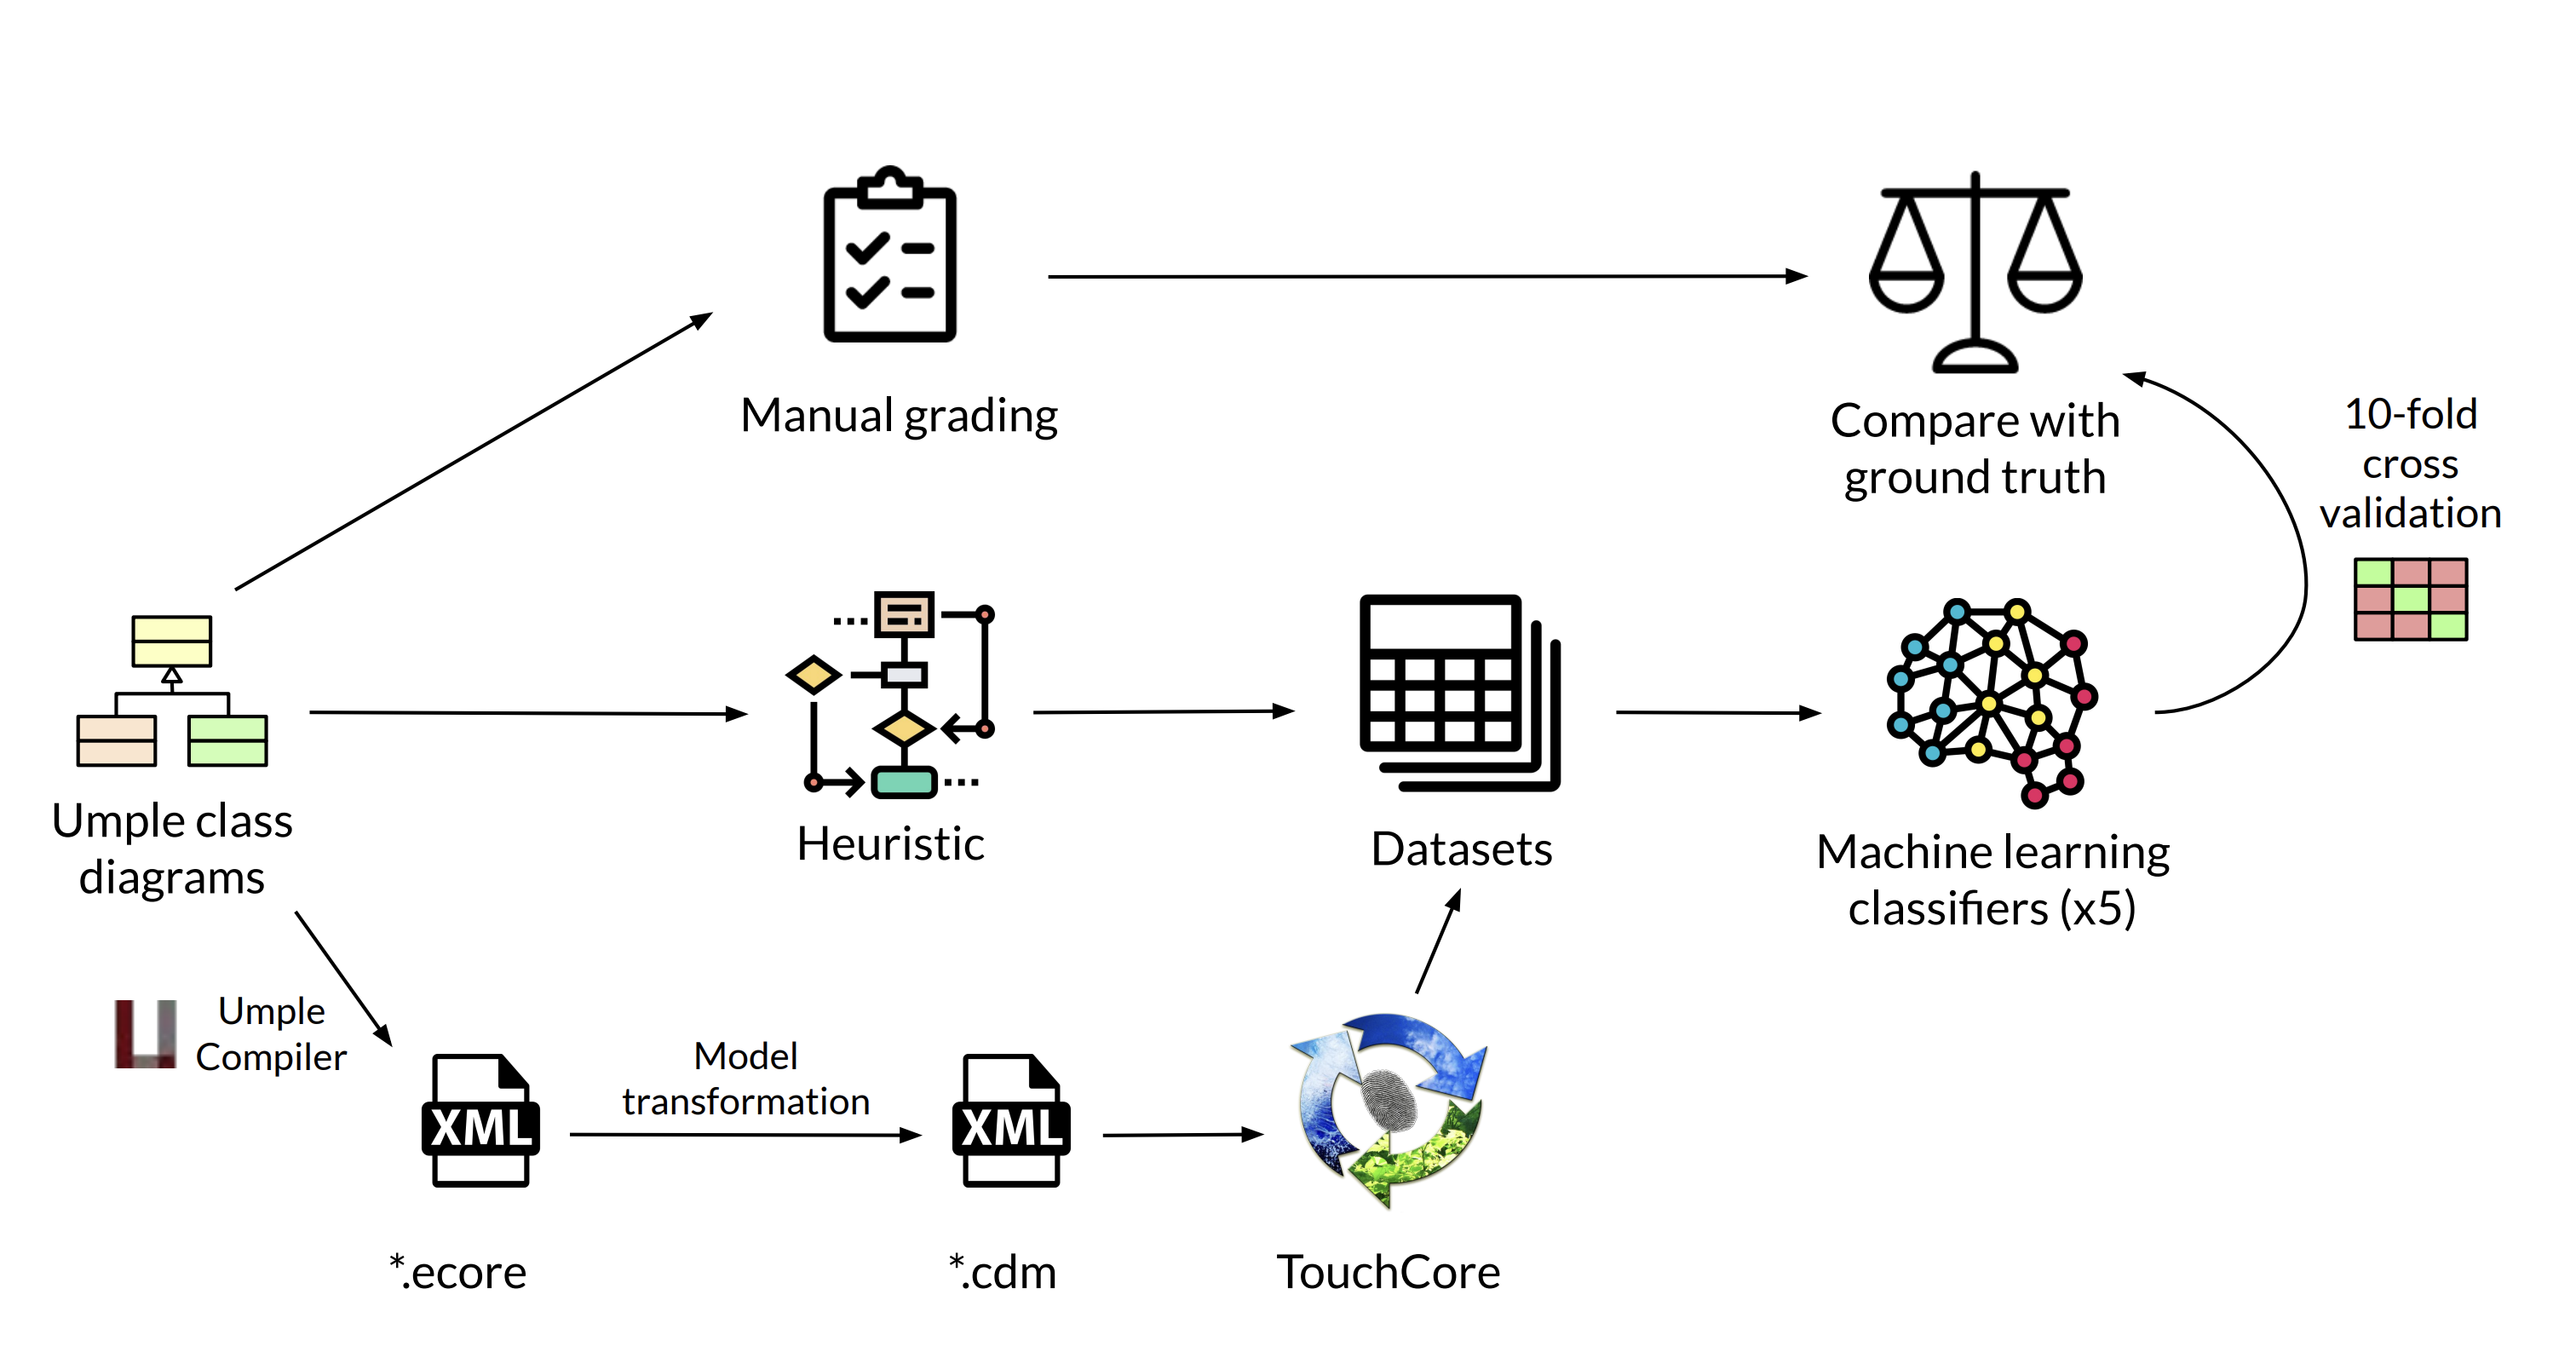
\includegraphics[width=14cm]{images/ml-approach.png}
	\caption{Ansatz der Studie \cite{boubekeur2020automatic}.}
	\label{fig:ml-approach}
\end{figure}

Um die Effektivität ihres vorgeschlagenen Ansatzes zu validieren, führten die Autoren eine empirische Studie mit 50 Studierenden durch, die an einem Softwaretechnikkurs teilnahmen. Die Studierenden wurden gebeten, UML-Diagramme für ein gegebenes Problem einzureichen, und die Autoren wandten ihren innovativen Ansatz zur Bewertung dieser Einreichungen an. Um die Zuverlässigkeit der Bewertung sicherzustellen, wurden auch zwei menschliche Prüfer beauftragt, dieselben Einreichungen unabhängig voneinander zu bewerten.

Die Ergebnisse der Studie zeigen, dass der vorgeschlagene Ansatz mit der menschlichen Bewertung hinsichtlich der Identifizierung hochwertiger Einreichungen vergleichbar ist und erstaunlich präzise ungefähre Noten vorhersagen kann. Darüber hinaus verglichen die Autoren ihren Ansatz mit einer komplexen regelbasierten Technik und stellten fest, dass ihre Methode in Bezug auf Effizienz und Wartbarkeit überlegen ist \cite{boubekeur2020automatic}.

Zusammenfassend bietet der innovative Ansatz eine vielversprechende Lösung zur Bewertung von UML-Diagrammen im Bereich der Softwaretechnikausbildung. Durch die Kombination eines einfachen heuristischen Algorithmus mit fortgeschrittenen maschinellen Lernverfahren identifiziert ihr Ansatz nicht nur hochwertige Einreichungen, sondern bietet auch eine effiziente Möglichkeit zur Vorhersage ungefährer Noten. Die Autoren betonen das potenzielle Zeitersparnis und die Reduzierung der Subjektivität im Bewertungsprozess und schlagen vor, dass ihr Ansatz auf andere Bereiche erweitert werden kann, sofern es eine klare Definition einer Idealvorlage gibt und eine Methode existiert, um die Einreichungen der Studierenden mit dieser Idealvorlage zu vergleichen.


\subsection{Bewertung auf Basis von Ähnlichkeitsmaßen}

Die Autoren des Artikels ``A Different Approach on Automated Use Case Diagram Semantic Assessment'' \cite{fauzan2021different} sind Daniel Siahaan, Siti Rochimah, Reza Fauzan und Evi Triandini. In diesem Artikel stellen die Autoren eine innovative Methode zur automatischen semantischen Bewertung von Anwendungsfall-Diagrammen im Rahmen von UML-Diagrammen vor. Das Hauptziel dieser Methode besteht darin, die Herausforderungen anzugehen, vor denen Pädagogen bei der Bewertung von Anwendungsfall-Diagrammen stehen, sowohl in zwischenmenschlicher als auch intrapersonaler Hinsicht.

Die Autoren verwenden einen semantischen Bewertungsansatz, der in zwei Hauptdimensionen unterteilt ist: Eigenschaft (property) und Beziehung (relationship). Alle in dieser Bewertung verwendeten Informationen stammen aus Beschriftungen, die aus einem \ac{XMI}-Dokument \cite{xmi} übersetzt wurden. Zur Messung der Ähnlichkeit zwischen den Beschriftungen verwenden die Autoren die Kosinus-Ähnlichkeit und nutzen WuPalmer zur Unterstützung von WordNet-Suchen \cite{fauzan2021different}.

Für ihre empirische Studie sammelten die Autoren einen Datensatz aus drei unterschiedlichen Projekten: Outlay, QuickBill und dem Restaurant Management System (RMS). Diese Projekte umfassen die Finanzaufzeichnung, den Point of Sale und das Restaurant-Bestellsystem. Der Quellcode für diese Projekte wurde von GitHub bezogen und folgt einem objektorientierten Ansatz. Den Studierenden wurden Demonstrationen zur Funktionsweise jedes Projekts gezeigt, und anschließend wurden sie aufgefordert, Anwendungsfall-Diagramme auf der Grundlage ihres Verständnisses der Projekte und der zugehörigen Terminologie zu erstellen. Insgesamt sammelten die Autoren 36 Anwendungsfall-Diagramme von den Studierenden, wobei jedes Projekt ein Antwortschlüssel-Diagramm hatte. Somit umfasst der Datensatz insgesamt 39 Anwendungsfall-Diagramme \cite{fauzan2021different}.

Bevor sie ihre vorgeschlagene Methode bewerteten, etablierten die Autoren einen Goldstandard als Referenz für die Bewertung. Dieser Goldstandard repräsentiert das durchschnittliche Ergebnis der Expertenbewertungen von Studentenantworten auf der Grundlage des Antwortschlüssels. Insgesamt beteiligten sich 21 Experten an dieser Bewertung, die von zwölf verschiedenen Universitäten stammten. Die Mindestanforderung für eine Expertin oder einen Experten war ein Master-Abschluss in Informatik.

Zur Bewertung ihrer vorgeschlagenen Methode nutzten die Autoren Gwets AC1, ein Maß, das den Grad der Übereinstimmung zwischen zwei Experten anzeigt. In diesem Fall repräsentiert der erste Experte den Durchschnitt der Bewertungen der Experten, während der zweite Experte die Bewertung durch die vorgeschlagene Methode darstellt. Die Autoren übertrugen die Ähnlichkeitswerte der beiden Experten auf eine Skala von 1 bis 5, wobei eine Wertung von eins ein Bewertungsergebnis von weniger als zwanzig, zwei ein Bewertungsergebnis von zwanzig bis vierzig, drei ein Ergebnis von vierzig bis sechzig, vier ein Ergebnis von sechzig bis achtzig und fünf ein Ergebnis von mehr als achtzig darstellt. Anschließend berechneten die Autoren die Übereinstimmung zwischen den beiden Experten unter Verwendung von Gwets AC1 \cite{fauzan2021different}.

Die Ergebnisse ihrer Bewertung zeigten, dass die vorgeschlagene Methode eine erhebliche Übereinstimmung mit der Bewertung durch den Experten aufwies. Interessanterweise stellten die Autoren fest, dass ihre vorgeschlagene Methode eine höhere Übereinstimmung mit dem Experten aufwies als die durchschnittliche Übereinstimmung zwischen den Experten. Darüber hinaus beobachteten die Autoren, dass Pädagogen tendenziell mehr Wert auf Informationen über Eigenschaften legen als auf Informationen über Beziehungen bei der Bewertung von Anwendungsfall-Diagrammen. Diese Erkenntnis könnte dazu beitragen, den Bewertungsprozess zu verbessern und eine konsistentere und objektivere Bewertung von Studentenantworten zu gewährleisten \cite{fauzan2021different}.

Zusammenfassend stellen die Autoren eine innovative Methode zur automatischen semantischen Bewertung von Anwendungsfall-Diagrammen vor. Ihr Ansatz umfasst die semantische Bewertung in den Dimensionen (property) und Beziehung (relationship), wobei ein Datensatz aus realen Projekten gesammelt und ein Goldstandard als Referenz etabliert wurde. Die Evaluation ihrer Methode unter Verwendung von Gwets AC1 zeigt eine erhebliche Übereinstimmung mit Expertenbewertungen. Darüber hinaus liefert ihre Erkenntnis darüber, dass Pädagogen bei der Bewertung von Anwendungsfall-Diagrammen tendenziell Eigenschaftsinformationen stärker gewichten als Beziehungsinformationen, wertvolle Einblicke zur Verbesserung des Bewertungsprozesses und zur Förderung einer konsistenteren und objektiveren Bewertung von Studentenantworten.

\subsection{Graph matching zur Bewertung von UML}

Der Artikel mit dem Titel ``New method for summative evaluation of UML class diagrams based on graph similarities'' wurde von Outair Anas, Mohammed Ouadou und Abdelhadi Lotfi verfasst \cite{anas2021new}. In ihrem Artikel widmen sich die Autoren der anspruchsvollen Aufgabe der Bewertung von UML-Klassendiagrammen, die von Studierenden erstellt wurden. Diese Aufgabe ist oft komplex für Lehrende, da UML-Klassendiagramme mehrere gültige Darstellungen haben können. Die Autoren schlagen ein halbautomatisches System vor, das dieses Problem durch den Einsatz eines Vergleichs von syntaktischen, strukturellen und semantischen Ähnlichkeiten angeht, um Fehler von Studierenden zu identifizieren und wertvolles Feedback zu ihrem Lernprozess zu geben. Ihre Methode besteht aus drei Schritten: 

\begin{enumerate}
    \item \textbf{UML-Diagramme in Graphen umwandeln:} Die Autoren beginnen ihren Ansatz, indem sie UML-Klassendiagramme in Graphdarstellungen umwandeln und das Metamodell durch die Einführung neuer Elemente zur Erleichterung der Bewertung verbessern. Sie stellen Klassen als Knoten dar, Attribute als mit Klassen verbundene Knoten und Assoziationen als beschriftete Kanten \cite{auxepaules2015diagram}.

    \item \textbf{Definition von Ähnlichkeitsmaßen:} Die Autoren definieren eine Reihe von Ähnlichkeitsmaßen, die auf die transformierten UML-Graphen anwendbar sind. Sie untersuchen verschiedene Techniken zur Graphabstimmung und Metriken zur Knotenähnlichkeit, um den Vergleich von Graphen und die Fehlererkennung zu erleichtern \cite{fauzan2018class}.

    \item \textbf{Abgleich und Vergleich von Graphen:} Unter Verwendung der zuvor definierten Ähnlichkeitsmaße führen die Autoren einen Abgleich und Vergleich der von Studierenden erstellten UML-Diagramme und der vom Lehrer bereitgestellten Referenzdiagramme durch \cite{outair2017towards} (Siehe \ref{fig:graph-matching}).
\end{enumerate}


\begin{figure}
	\centering
	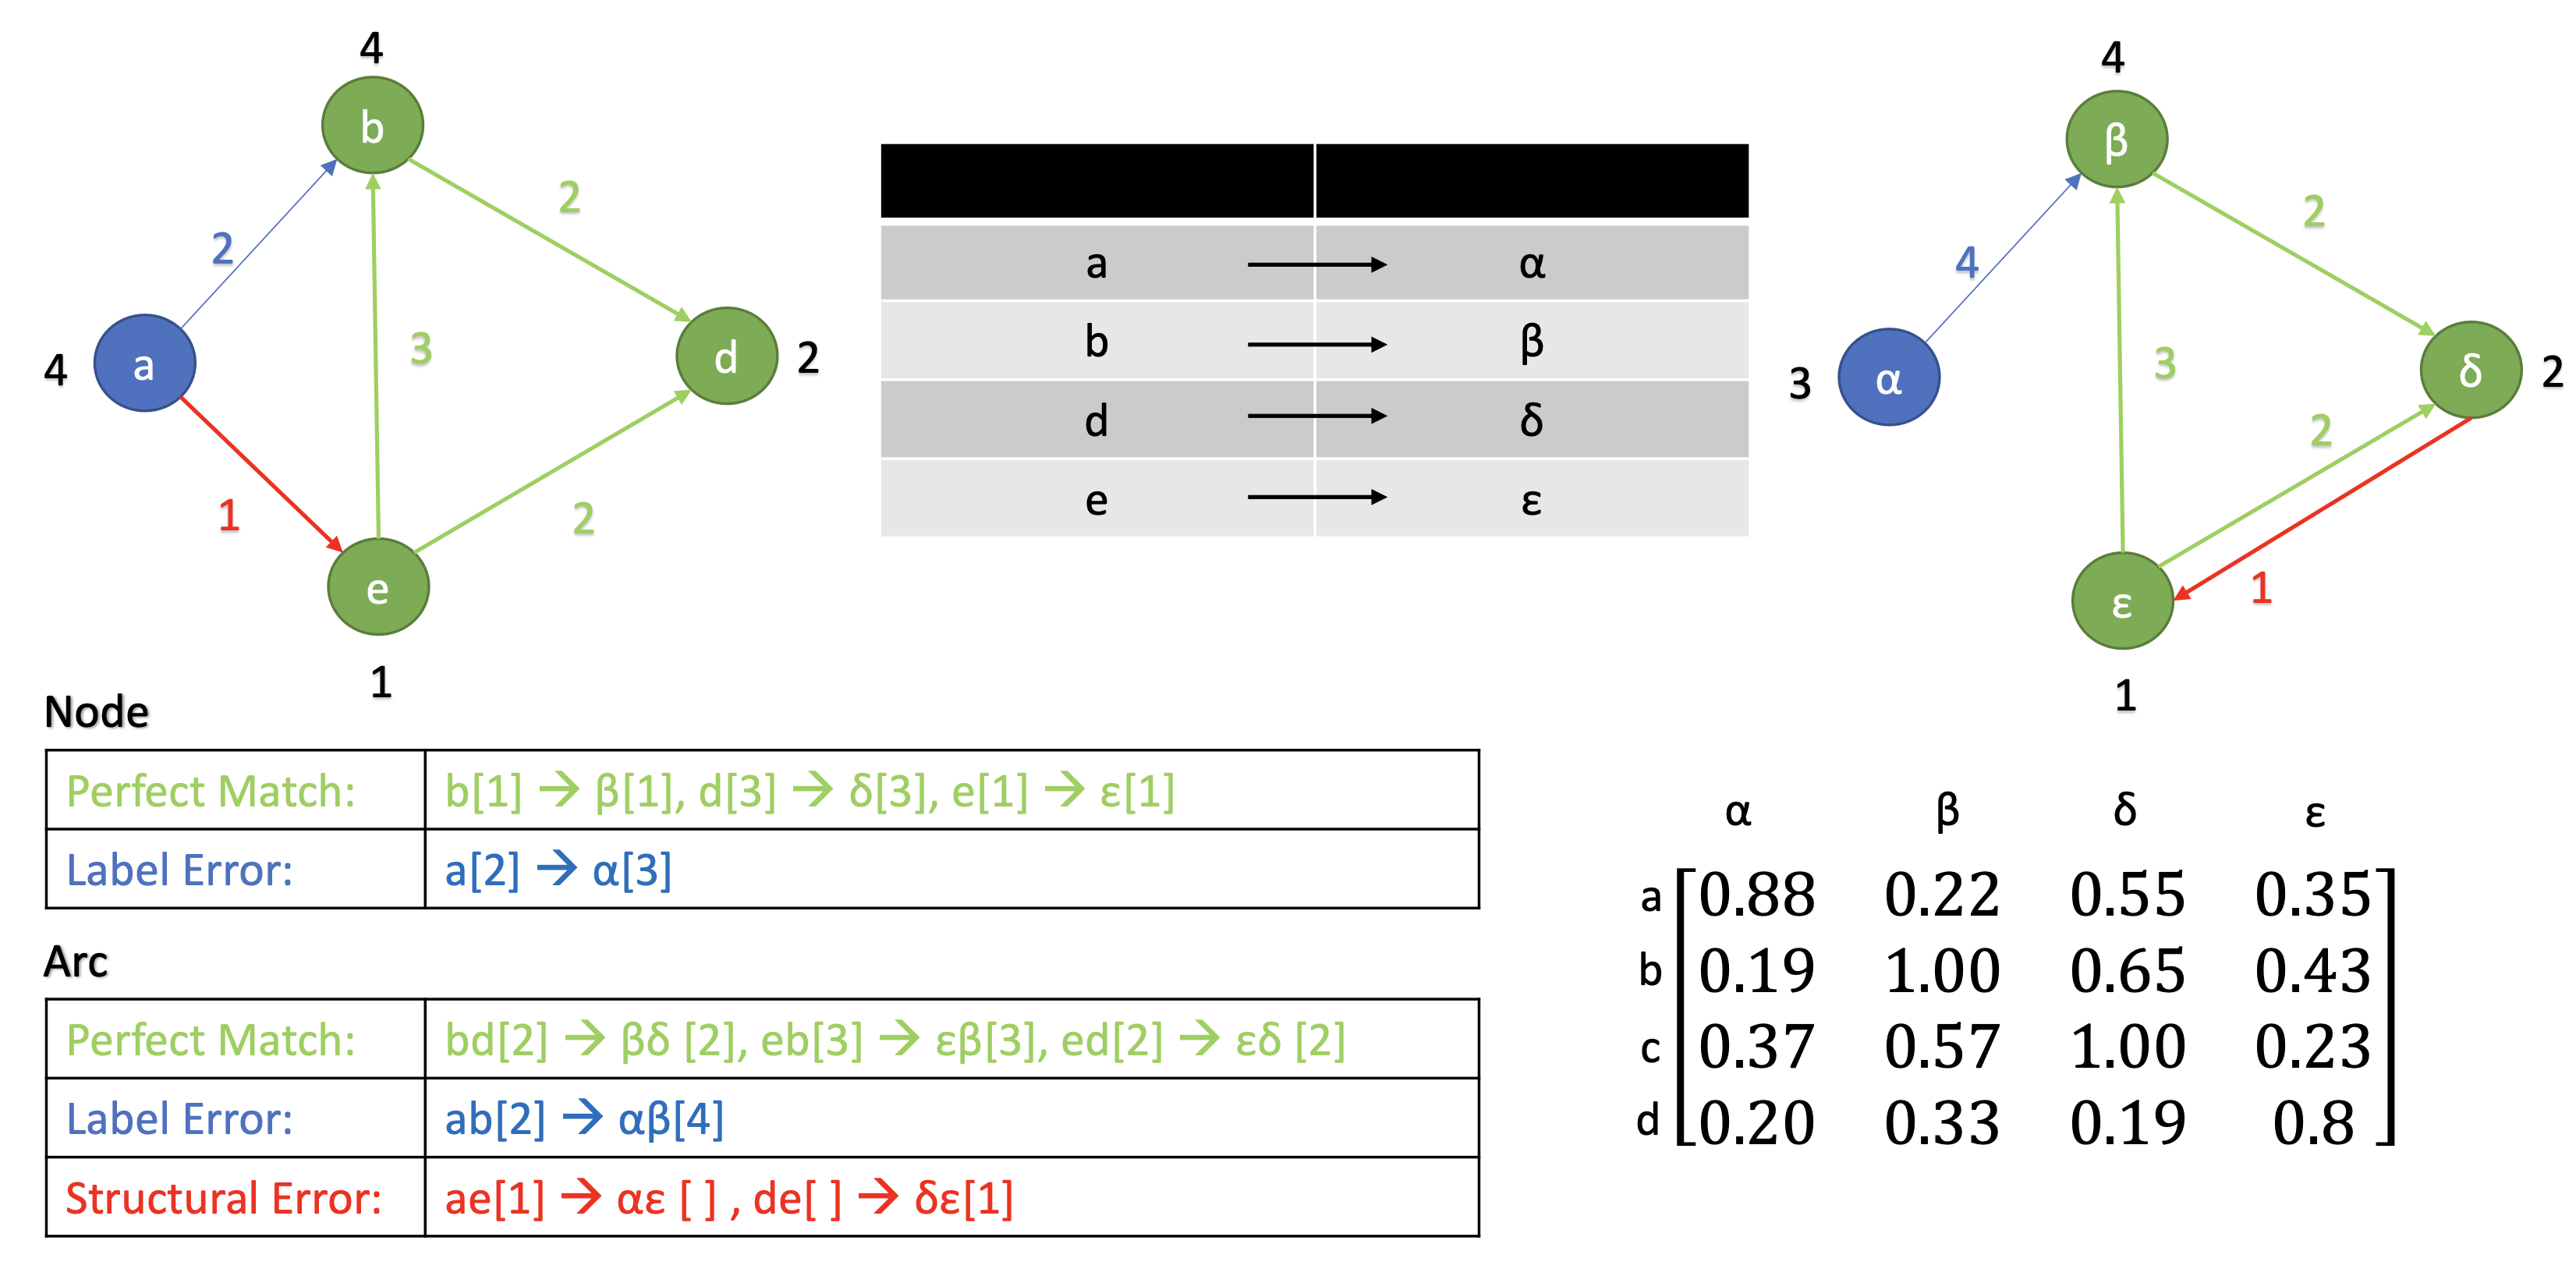
\includegraphics[width=15cm]{images/graph-matching.png}
	\caption{Beispiel für einen Graphenabgleich \cite{anas2021new}.}
	\label{fig:graph-matching}
\end{figure}

Die Leistung des Systems wird anhand eines Datensatzes bewertet, der aus 100 von Studierenden erstellten Klassendiagrammen besteht, wobei für jedes Diagramm ein entsprechendes Referenzdiagramm zur Bewertung bereitgestellt wird. Drei Übungen werden ausgewählt, um das System offline zu konfigurieren und zu bewerten, wobei iterative Verbesserungen an den Ähnlichkeitskriterien und der Systemfunktionalität auf Grundlage der Übungsergebnisse vorgenommen werden. Die Ergebnisse zeigen, dass das System eine Genauigkeitsrate von 70 \% bei der Erkennung von Fehlern von Studierenden erreicht und minimalen Eingriff erfordert, um Übereinstimmungen für 80 \% der verarbeiteten Diagramme zu korrigieren \cite{anas2021new}. Die Autoren betonen, dass der in das System integrierte formative Bewertungsansatz gut geeignet ist, um UML-Klassendiagramme zu bewerten, da er den Studierenden Feedback zur Verbesserung ihres Verständnisses des Lehrstoffes liefert. Darüber hinaus hat das System das Potenzial, die Belastung der Lehrenden zu verringern, indem es den Bewertungsprozess automatisiert und ihnen ermöglicht, individuelleres Feedback an einzelne Studierende zu geben.

Zusammenfassend bietet die in diesem Artikel vorgestellte Methode eine vielversprechende Möglichkeit zur summativen Bewertung von UML-Klassendiagrammen unter Berücksichtigung der Möglichkeit mehrerer gültiger Darstellungen. Durch den umfassenden Vergleich von syntaktischen, strukturellen und semantischen Ähnlichkeiten kann das System Fehler in von Studierenden erstellten Diagrammen erkennen und zur Verbesserung ihres Lernfortschritts beitragen. Die Autoren erkennen an, dass weitere Forschung erforderlich ist, um das System zu verfeinern und seine Genauigkeit zu verbessern, aber die Ergebnisse dieser Studie legen nahe, dass es das Potenzial hat, eine wertvolle Unterstützung sowohl für Lehrende als auch für Studierende bei der Bewertung von UML-Klassendiagrammen zu sein.

\subsection{Automatisierte Bewertung mit GReQL}

In ihrem Artikel ``Automated checks on UML diagrams'' \cite{striewe2011automated} stellen Michael Striewe und Michael Goedicke eine innovative Technik zur Evaluierung von UML-Klassendiagrammen auf der Grundlage von Graphabfragen vor. Sie betrachten UML-Klassendiagramme als Graphen und formalisieren ihren Ansatz mithilfe einer Graphabfragesprache namens GReQL, die von der JGraLab-Bibliothek bereitgestellt wird.

\ac{GReQL}, ähnlich wie SQL, eignet sich gut für die Implementierung regelbasierter Prüfungen von graphenbasierten Daten \cite{striewe2014automated}. Sie ermöglicht die Abfrage von Elementen bestimmter Typen, die Untersuchung ihrer Verbindungen und die Überprüfung ihrer Attribute. Im Kontext von UML-Klassendiagrammen können diese Abfragen das Vorhandensein von Diagrammelementen wie Klassen, Schnittstellen, Eigenschaften, Operationen, Parametern, Assoziationen und Generalisierungen ermitteln und ihre Beziehungen bewerten \cite{striewe2011automated}.

\begin{lstlisting}[caption={[Codebeispiel] Codebeispiel in GReQL}, label=code:GreQL, float=!ht, language=xml]
  <rule type="presence" points="5">
    <query>
    from x : V{Class},
    y : V{Property}, z : V{PrimitiveType}
           with
              isDefined(x.name) and x.name="A" and
              x --> y and
              isDefined(y.name) and y.name="b" and
              y --> z and
              isDefined(z.name) and z.name="String"
           report 1 end
    </query>
    <feedback>Ein "A" soll ein Attribut für die
    Eigenschaft "b" bereitstellen.</feedback>
  </rule>
\end{lstlisting}

Um ein UML-Diagramm mithilfe dieses Ansatzes zu evaluieren, parsen die Autoren das Diagramm zunächst in eine graphenbasierte Darstellung seiner abstrakten Syntax, in der Regel durch einen XML-Parser. Anschließend verwenden sie \ac{GReQL}-Abfragen, um die Anwesenheit bestimmter Diagrammelemente und ihrer Verbindungen zu überprüfen. Die Autoren stellen eine Reihe von Regeln vor, die als \ac{GReQL}-Abfragen implementiert sind und an die Anforderungen bestimmter Kurse oder Aufgaben angepasst werden können.

In ihrem Bewertungssystem werden einzelnen Regeln individuelle Punktzahlen zugewiesen, wobei unterschiedliche Gewichtungen zur Unterscheidung zwischen Korrektheits- und Qualitätsaspekten verwendet werden. Zum Beispiel könnte eine Regel, die das Vorhandensein einer Klasse mit einem bestimmten Namen sicherstellt, als wichtiger angesehen werden als eine, die das Vorhandensein eines Kommentars zu einer Klasse überprüft. Die Autoren schlagen auch eine Methode zur Berechnung von Gesamtnoten vor, indem die Punktzahlen jeder Regel aggregiert werden \cite{striewe2011automated}.

Um die praktische Anwendung ihres Ansatzes zu zeigen, bieten die Autoren ein Beispiel aus einem UML-Modellierungskurs an, in dem Lösungen von Studierenden automatisch mit ihrer Methodik bewertet wurden. Das Ergebnis dieser Beispielbewertung zeigt die Effektivität ihres Ansatzes bei der Erkennung von Fehlern und der Bereitstellung rechtzeitigen Feedbacks an die Studierenden, wodurch die Arbeitsbelastung der Dozenten reduziert wird \cite{striewe2011automated}.

Über UML hinaus sehen die Autoren die Vielseitigkeit ihres Ansatzes bei der Bewertung anderer Sprachen, die in eine graphenbasierte Darstellung ihrer abstrakten Syntax transformiert werden können, was praktisch alle Programmiersprachen einschließt. Sie sehen seine Anwendung in intelligenten Tutoringsystemen und automatisiertem Tutoring, da es eine sofortige Rückmeldung an Studierende ermöglicht und den Bewertungsprozess für Lehrkräfte vereinfacht.

Mögliche Einschränkungen dieses Ansatzes sind jedoch die Abhängigkeit von der Annahme einer korrekten Umwandlung von UML-Diagrammen in graphenbasierte Darstellungen, die zu Ungenauigkeiten führen kann, wenn der Umwandlungsprozess fehlerhaft ist. Die Autoren schlagen jedoch vor, den Umwandlungsprozess durch eine Reihe von Testfällen zu validieren, um die Zuverlässigkeit sicherzustellen \cite{striewe2011automated}.

Zusätzlich konzentriert sich der Ansatz hauptsächlich darauf, das Vorhandensein von Diagrammelementen und ihren Verbindungen zu überprüfen, bewertet jedoch nicht intrinsisch die Korrektheit des Inhalts innerhalb dieser Elemente. Zum Beispiel kann er überprüfen, ob eine Klasse einen bestimmten Namen hat, aber er überprüft nicht die Richtigkeit der zugehörigen Attribute und Methoden. Die Autoren weisen jedoch darauf hin, dass ihr Ansatz erweitert werden kann, um komplexere Regeln für die Bewertung des Inhalts von Diagrammelementen zu umfassen \cite{striewe2014automated}.

Zusammenfassend bietet der Ansatz von Striewe und Goedicke eine vielversprechende Alternative zur Bewertung von UML-Klassendiagrammen. Indem sie diese Diagramme als Graphen behandeln und \ac{GReQL} für Abfragen nutzen, bieten sie eine flexible und anpassbare Möglichkeit zur Bewertung. Ihre Methodik hat das Potenzial für breitere Anwendungen in verschiedenen Sprachen und Bildungsbereichen und verspricht, das Feedback an Studierende zu verbessern, während sie die Arbeit für Lehrende vereinfacht.


\section{JACK}

Das E-Assessment-System namens ``JACK3'' (dritte Version von JACK) \cite{jack}, entwickelt von der Universität Duisburg-Essen, stellt eine webbasierte Plattform dar, die Pädagogen eine effektive Lösung für die Erstellung und Durchführung von Online-Übungen bietet. Diese vielseitige Plattform ermöglicht Lehrkräften die Erstellung einer breiten Palette von Übungen, die nahtlos über eine benutzerfreundliche Oberfläche bereitgestellt werden können. Neben der Erstellung von Bewertungen verfügt JACK3 über eine Auswahl an Funktionen, die den Bewertungsprozess optimieren sollen. Diese beinhalten die automatisierte Bewertung, umfassende Berichterstellungswerkzeuge und die Echtzeitverfolgung des Lernfortschritts der Schüler.

Die Bedeutung von JACK3 reicht über die reine Bequemlichkeit hinaus, da es Lehrern ermöglicht, wertvolle Zeit und Ressourcen zu sparen, während gleichzeitig die Effizienz und Effektivität der Bewertungen gesteigert werden. Des Weiteren bereichert JACK3 das Lernerlebnis, indem es den Schülern ansprechende und personalisierte Bewertungen bietet, begleitet von sofortigem Feedback. Die Plattform erleichtert die Datensammlung zur Überwachung des Lernfortschritts der Schüler und zur Identifizierung von Verbesserungsmöglichkeiten. Sie unterstützt verschiedene Lehr- und Lernmethoden, darunter das umgekehrte Klassenzimmer, Blended Learning und Fernunterricht \cite{jack}.

Darüber hinaus bietet JACK3 eine Vielzahl weiterer Vorteile, wie die Steigerung der Schülerbeteiligung und -motivation, die Möglichkeit zur schnellen Bewertung und Rückmeldung von Aufgaben sowie die Prävention von Betrug und Plagiat. Zusätzlich bietet es erweiterte Möglichkeiten zur Verfolgung der Schulentwicklung. JACK3 bietet eine breite Palette von Übungstypen an, die den unterschiedlichen Lernzielen der Pädagogen und den spezifischen Bedürfnissen ihrer Schüler gerecht werden. Zu den Beispielen gehören Multiple-Choice-Quizfragen, Wahr/Falsch-Quizfragen, Zuordnungsübungen, Lückentextübungen, Kurzantwortfragen Aufsatzfragen und vieles mehr. Des Weiteren ermöglicht JACK3 die Erstellung komplexerer Übungen wie Drag-and-Drop-Aufgaben, Hotspot-Übungen, Umfragen zur Datensammlung und Webquests, die eine tiefgehende Exploration von Themen ermöglichen \cite{jack}.

Es ist erwähnenswert, dass JACK3 seine Fähigkeiten zur Unterstützung der Bewertung von Übungen zur Unified Modeling Language (UML) erweitert hat, was seine Anwendbarkeit in der Softwaretechnik-Ausbildung verbessert. Lehrer können das System nutzen, um UML-Diagramme wie Klassendiagramme, Sequenzdiagramme und Aktivitätsdiagramme automatisch zu bewerten.

Im Bereich der UML-Übungen bietet JACK3 Lehrern die Flexibilität, Übungen zu gestalten, die Klassendiagramme, Sequenzdiagramme und Aktivitätsdiagramme umfassen. Diese Übungen ermöglichen es den Schülern, die Struktur und das Verhalten von Softwaresystemen zu visualisieren, die komplexen Beziehungen zwischen Systemkomponenten zu verstehen, ihre Ideen effektiv an Kommilitonen zu kommunizieren und ihre Fähigkeiten im Bereich Problemlösung und kritisches Denken zu schärfen \cite{jack}.


Das Hauptaugenmerk dieser wissenschaftlichen Arbeit liegt auf der Analyse und Evaluierung des Instrumentariums JACK, insbesondere seiner Kapazität zur kritischen Beurteilung von UML-Diagrammen. Im darauf folgenden Abschnitt wird die spezifische Problematik in umfassender Weise erörtert und eine breite Palette möglicher Lösungsansätze erörtert.